\documentclass[11pt,a4paper]{article}
\usepackage[utf8]{inputenc}
\usepackage[T1]{fontenc}
\usepackage[brazil]{babel}
\usepackage{lmodern}
\usepackage{microtype}
\usepackage[margin=2.3cm]{geometry}
\usepackage{amsmath}
\usepackage{booktabs}
\usepackage{graphicx}
\usepackage{xcolor}
\usepackage{listings}
\usepackage{float}
\usepackage{enumitem}
\usepackage[hidelinks]{hyperref}

\definecolor{fundo}{HTML}{F6F7F9}
\definecolor{coment}{HTML}{5F7A61}
\definecolor{palavra}{HTML}{1F4E9C}
\lstdefinelanguage{APDL}{
  morekeywords={ET,MP,SECTYPE,SECDATA,LESIZE,LMESH,D,F,FDELE,FCUM,NMODIF,MODMSH,
    SOLVE,NLGEOM,NSUBST,AUTOTS,STABILIZE,LNSRCH,TIME,OUTRES,ANTYPE,SET,ETABLE,
    *DO,*ENDDO,*IF,*ENDIF,*ELSEIF,*GET,*DIM,*VWRITE,*CFOPEN,*CFCLOS,FINISH,ALLSEL,CNVTOL},
  sensitive=false, comment=[l]{!}, morestring=[b]"
}
\lstset{
  basicstyle=\ttfamily\small, backgroundcolor=\color{fundo}, frame=single, rulecolor=\color{gray!40},
  keywordstyle=\color{palavra}\bfseries, commentstyle=\color{coment}\itshape,
  breaklines=true, columns=fullflexible, keepspaces=true, xleftmargin=4pt, xrightmargin=4pt,
  literate={á}{{\'a}}1 {à}{{\`a}}1 {ã}{{\~a}}1 {â}{{\^a}}1 {é}{{\'e}}1 {ê}{{\^e}}1 {í}{{\'i}}1
           {ó}{{\'o}}1 {õ}{{\~o}}1 {ô}{{\^o}}1 {ú}{{\'u}}1 {ç}{{\c c}}1 {Ç}{{\c C}}1 {É}{{\'E}}1 {Á}{{\'A}}1
}

\title{\textbf{Simulação numérica (Ansys MAPDL) do Estudo de Caso \#3}\\[4pt]
\large O que é cada arquivo, o que faz cada bloco do código e por que cada escolha foi feita}
\author{Material de apoio ao TCC --- Armellini \& Rüher Vicente}
\date{Setembro de 2026}

\begin{document}
\maketitle
\tableofcontents

% =====================================================================
\section{Visão geral}

O objetivo da simulação é reproduzir, pelo Método dos Elementos Finitos, o Estudo de Caso \#3 do TCC:
três trechos de cabo ancorados em $A$, $B$ e $C$ e ligados num nó livre $P$, sob peso próprio.
O modelo analítico trata cada trecho como uma catenária de um \emph{cabo ideal}: inextensível e com
rigidez à flexão nula. O desafio do modelo numérico é aproximar esse cabo ideal com os elementos
disponíveis no Ansys e ainda assim convergir.

O fluxo de trabalho é:
\begin{enumerate}[itemsep=2pt]
  \item \texttt{catenaria3d.inp} --- modelo APDL do caso principal (geometria, malha, cargas, solução
        não linear, pós-processamento). Pode ser rodado sozinho no Ansys.
  \item \texttt{exportar\_resultados.inp} --- roda o modelo acima e exporta, para todos os subpassos,
        coordenadas, deslocamentos e esforços, que alimentam o visualizador web.
  \item \texttt{estudo\_rigidez.py} --- estudo paramétrico da rigidez à flexão (Seção~\ref{sec:estudo}).
  \item \texttt{casos\_forca.py} --- gera e roda os casos com força concentrada (Seção~\ref{sec:casos}).
\end{enumerate}

\begin{table}[H]
\centering
\caption{Arquivos da pasta \texttt{ansys/} do repositório.}
\begin{tabular}{p{5.3cm}p{9.7cm}}
\toprule
\textbf{Arquivo} & \textbf{Para que serve} \\
\midrule
\texttt{catenaria3d.inp} & Modelo APDL do caso principal (versão final, corrigida). \\
\texttt{exportar\_resultados.inp} & Macro APDL que roda o modelo e exporta os resultados de todos os subpassos. \\
\texttt{estudo\_rigidez.py} & Varre o momento de inércia da seção e compara com o modelo analítico. \\
\texttt{casos\_forca.py} & Gera, roda e converte os casos com força concentrada. \\
\texttt{rodar\_exportacao.ps1} & Roda o modelo no Ansys e gera os dados do visualizador. \\
\texttt{figuras\_mef.py} & Gera as figuras do capítulo de elementos finitos do TCC. \\
\texttt{exemplos/exemplo\_caso\_forca\_CP\_45pct\_1000N.inp} & Exemplo completo de \texttt{.inp} gerado pelo \texttt{casos\_forca.py} (força de 1000~N a 45\% do cabo C--P). \\
\bottomrule
\end{tabular}
\end{table}

Todos os arquivos estão no repositório público do trabalho,
\url{https://github.com/HenriqueRuher/tcc-estruturas-cabos}, junto com os códigos analíticos e o
visualizador, que também pode ser aberto diretamente no navegador em
\url{https://henriqueruher.github.io/tcc-estruturas-cabos/}.

% =====================================================================
\section{O modelo \texttt{catenaria3d.inp}, bloco a bloco}

\subsection{Parâmetros e geometria}
Os parâmetros são os da Tabela~4.13 do TCC ($y$ é a vertical):
\begin{lstlisting}[language=APDL]
xa=0     $ ya=20    $ za=0
xb=40    $ yb=20    $ zb=0
xc=20    $ yc=15    $ zc=25
L1=50 $ LC=30 $ eta=0.5 $ LA=eta*L1 $ LB=(1-eta)*L1
q1=40 $ q2=20
xp0=(xa+xb)/2 $ yp0=10 $ zp0=8      ! palpite inicial de P
\end{lstlisting}
Cria-se uma linha reta de cada ancoragem até o palpite de $P$. Essas linhas só servem para gerar a
malha; os nós são depois reposicionados na forma inicial curva (Seção~\ref{sec:forma}).

\subsection{Elemento: por que \texttt{BEAM188} e não \texttt{LINK180}}
O elemento mais próximo de um cabo ideal no Mechanical APDL clássico seria o \texttt{LINK180}
(treliça: só força axial). Ele foi testado de várias formas (chute inicial exato, pré-tensão
térmica, malha mais grossa etc.) e \textbf{não convergiu}: uma cadeia de barras articuladas sem
tração não tem rigidez transversal nenhuma, e a matriz de rigidez fica singular no início da solução.
O Mechanical APDL clássico não tem um elemento de cabo dedicado.

A solução foi usar o \texttt{BEAM188} (viga) com uma rigidez à flexão \emph{muito pequena}: ela só
existe para dar estabilidade numérica e deve influenciar o resultado o mínimo possível.

\subsection{Seção: área de 1 cm de raio, inércia reduzida}
Com uma seção circular maciça (\texttt{CSOLID}), área e inércia ficam acopladas: $A=\pi r^2$ e
$I=\pi r^4/4$. Diminuir o raio reduz a rigidez à flexão $EI$, mas também a rigidez axial $EA$.
Por isso a seção passou a ser genérica (\texttt{ASEC}), com $A$ e $I$ independentes:
\begin{lstlisting}[language=APDL]
rsec=0.01                              ! raio de referencia: 1 cm
fI=0.01                                ! fator de reducao da inercia
Asec=3.14159265359*rsec**2
Isec=fI*3.14159265359*rsec**4/4
SECTYPE,1,BEAM,ASEC
SECDATA,Asec,Isec,0,Isec,0,2*Isec      ! A, Iyy, Iyz, Izz, Iw, J
\end{lstlisting}
\begin{itemize}[itemsep=2pt]
  \item $EA = 200\,\text{GPa}\times 3{,}14\cdot10^{-4}\,\text{m}^2 \approx 6{,}3\cdot10^{7}$~N: com
        trações da ordem de 1000~N, a deformação axial é $\sim 2\cdot10^{-5}$, ou seja, o cabo é
        praticamente inextensível, como no modelo analítico.
  \item $EI = f_I\cdot 1571$~N$\cdot$m$^2$. Com $f_I=0{,}01$, $EI \approx 15{,}7$~N$\cdot$m$^2$.
        É o menor valor que converge de forma confiável (Seção~\ref{sec:estudo}).
  \item As três seções são idênticas; ter três IDs só serve para saber depois, pelo número da seção,
        a qual trecho (A--P, B--P, C--P) cada elemento pertence.
\end{itemize}

\subsection{Malha e condições de contorno}
Cada trecho tem 40 elementos (\texttt{NDIV=40}): 120 elementos e 121 nós no total. As ancoragens
$A$, $B$ e $C$ são engastadas (\texttt{D,no,ALL,0}). O nó $P$ é livre e compartilhado pelos três
trechos, o que garante a continuidade (os três cabos se encontram em $P$).

\subsection{Forma inicial}\label{sec:forma}
Os nós são movidos (\texttt{NMODIF}) para uma parábola dentro do plano vertical de cada trecho, com
comprimento de arco igual ao comprimento do cabo ($L_A$, $L_B$, $L_C$) e profundidade maior que a da
solução. Ou seja, é um chute inicial propositalmente ruim, mas suave e sem pontos angulosos: o
objetivo é mostrar que a solução converge para o equilíbrio correto a partir de uma forma diferente
(a animação do visualizador mostra essa convergência). Chutes com ``quinas'' (zigue-zague,
triângulo) deixavam curvaturas residuais no resultado e foram descartados.

\subsection{Cargas: peso próprio pelo comprimento real de cada elemento}\label{sec:carga}
\textbf{Esta foi a correção mais importante.} Na versão anterior, cada nó recebia a mesma força
$q L/N_{div}$. Isso só é correto se todos os elementos tiverem o mesmo comprimento. Mas os nós da
parábola inicial não ficam igualmente espaçados ao longo do arco: os elementos têm de
$\approx 0{,}54$ a $\approx 0{,}81$~m. Na prática, o peso ficava distribuído por projeção, como numa
parábola, e não uniformemente ao longo do cabo, como na catenária.
Agora cada elemento recebe o peso do seu próprio comprimento, dividido entre os dois nós:
\begin{lstlisting}[language=APDL]
FDELE,ALL,ALL
FCUM,ADD                               ! forcas no mesmo no se SOMAM
*GET,emx,ELEM,0,NUM,MAX
*DO,e,1,emx
  n1=NELEM(e,1)
  n2=NELEM(e,2)
  *GET,sc,ELEM,e,ATTR,SECN             ! secao 3 = cabo C-P
  le=DISTND(n1,n2)                     ! comprimento real do elemento
  qe=q1
  *IF,sc,EQ,3,THEN
    qe=q2
  *ENDIF
  F,n1,FY,-qe*le/2
  F,n2,FY,-qe*le/2
*ENDDO
FCUM,REPL
\end{lstlisting}
Como o cabo é praticamente inextensível, o comprimento de cada elemento na forma inicial é o mesmo
na forma final, e a distribuição de peso fica correta.

\subsection{Solução não linear}
\begin{lstlisting}[language=APDL]
ANTYPE,STATIC
NLGEOM,ON                              ! grandes deslocamentos
AUTOTS,ON
NSUBST,200,20000,50                    ! subpassos: inicial, maximo, minimo
STABILIZE,REDUCE,ENERGY,1.0E-2
SOLVE
\end{lstlisting}
\begin{itemize}[itemsep=2pt]
  \item \texttt{NLGEOM,ON}: o equilíbrio de um cabo depende da própria forma deformada (não
        linearidade geométrica); sem isso não há catenária.
  \item O peso entra em rampa (fator de carga de 0 a 1) ao longo dos subpassos. Os subpassos
        \emph{não} são tempo físico: são passos do método numérico.
  \item \texttt{STABILIZE}: no início, com o cabo ainda sem tração, a rigidez transversal vem
        quase só do $EI$ pequeno e o sistema é quase singular. A estabilização adiciona um
        amortecimento artificial. Com a opção \texttt{REDUCE}, esse amortecimento vai a zero ao fim
        do passo de carga, e o equilíbrio final não é afetado. Isso foi conferido: com energia
        $10^{-2}$ e $10^{-1}$ o resultado final é idêntico.
\end{itemize}

\subsection{Pós-processamento}
São escritos: a posição final de $P$ (\texttt{resultado\_noP.txt}), a força axial de cada elemento
(\texttt{forcas\_linha*.txt}) e a tração horizontal $T_0$ no elemento junto a $P$
(\texttt{resumo\_T0.txt}), calculada como
\[
T_0 = N\,\frac{\sqrt{\Delta x^2+\Delta z^2}}{\sqrt{\Delta x^2+\Delta y^2+\Delta z^2}},
\]
isto é, a componente horizontal da força axial $N$ do elemento. Num cabo ideal só com cargas
verticais, $T_0$ é constante ao longo do trecho; no texto do TCC usa-se a média de $T_0$ na metade
central de cada trecho, longe das pequenas perturbações de flexão junto às extremidades.

% =====================================================================
\section{Estudo da rigidez à flexão}\label{sec:estudo}

O \texttt{estudo\_rigidez.py} gera cópias do modelo variando $f_I$ (com a área fixa), roda o Ansys
em lote em pastas temporárias e compara $P$ e $T_0$ com o modelo analítico. O estudo começou para
responder se reduzir a rigidez à flexão aproximaria a solução da analítica. Ao investigar por que
$T_0$ quase não mudava, apareceu a causa principal da diferença: a distribuição do peso
(Seção~\ref{sec:carga}).

\begin{figure}[H]
\centering
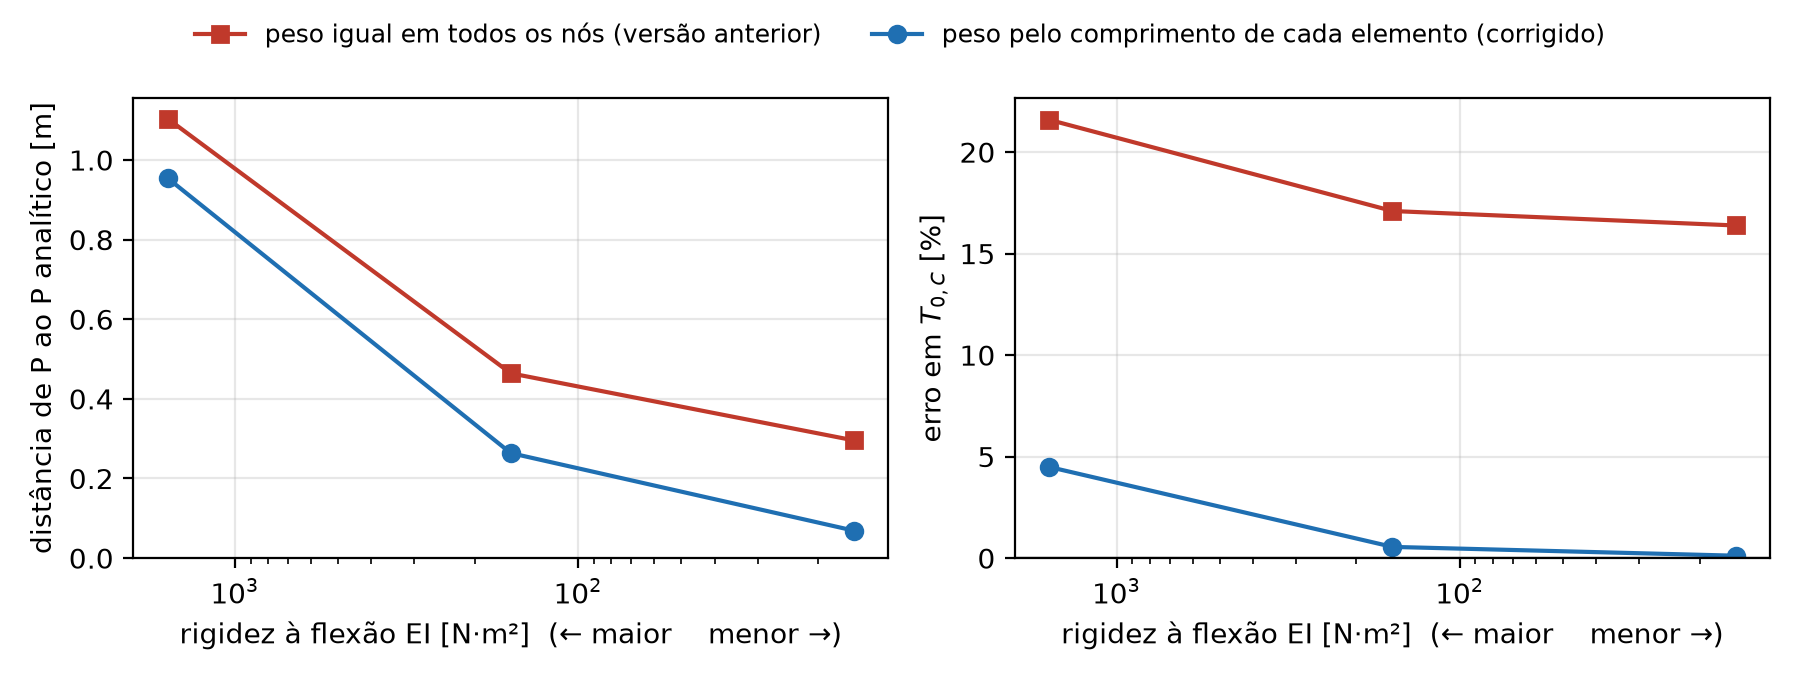
\includegraphics[width=\textwidth]{fig_estudo_rigidez.png}
\caption{Distância de $P$ ao $P$ analítico e erro em $T_{0,C}$ em função de $EI$, antes e depois da
correção da distribuição do peso.}
\label{fig:estudo}
\end{figure}

\begin{table}[H]
\centering
\caption{Resultados do caso principal (analítico: $P=(20{,}00;\,6{,}36;\,2{,}30)$~m,
$T_{0,A}=T_{0,B}=818{,}54$~N, $T_{0,C}=186{,}69$~N).}
\label{tab:estudo}
\begin{tabular}{lcccccc}
\toprule
\textbf{Peso nodal} & $\boldsymbol{EI}$ [N$\cdot$m$^2$] & $y_P$ [m] & $z_P$ [m] & $T_{0,A}$ [N] & $T_{0,C}$ [N] & $\Delta T_{0,C}$ \\
\midrule
igual em todos os nós & 1571 & 6,98 & 3,21 & 865,1 & 227,0 & +21,6\% \\
igual em todos os nós & 157  & 6,57 & 2,72 & 862,1 & 218,6 & +17,1\% \\
igual em todos os nós & 15,7 & 6,43 & 2,59 & 860,2 & 217,3 & +16,4\% \\
\midrule
por comprimento & 1571 & 6,97 & 3,03 & 818,6 & 195,1 & +4,5\% \\
por comprimento & 157  & 6,55 & 2,49 & 819,4 & 187,7 & +0,6\% \\
\textbf{por comprimento} & \textbf{15,7} & \textbf{6,41} & \textbf{2,34} & \textbf{818,7} & \textbf{186,9} & \textbf{+0,1\%} \\
\midrule
por comprimento & 1,57 & \multicolumn{5}{c}{não converge} \\
\bottomrule
\end{tabular}
\end{table}

Conclusões:
\begin{itemize}[itemsep=2pt]
  \item Com a carga corrigida e $EI=15{,}7$~N$\cdot$m$^2$ (modelo final), $T_0$ coincide com o
        analítico (0,0\% e +0,1\%) e $P$ fica a $\approx 7$~cm da posição analítica.
  \item O erro restante em $P$ diminui com $EI$ (aproximadamente com $\sqrt{EI}$, que é a escala do
        trecho junto às extremidades em que a flexão ainda atua).
  \item Abaixo de $EI\approx 15$~N$\cdot$m$^2$ o Newton-Raphson não converge nem com estabilização
        mais forte. Seria preciso outra estratégia (por exemplo, continuação em vários passos de
        carga), para um ganho de poucos centímetros.
  \item Com peso igual em todos os nós, reduzir $EI$ melhora $P$, mas $T_0$ para em $\approx +16\%$:
        o erro dominante era a distribuição do peso, não a rigidez à flexão.
\end{itemize}

% =====================================================================
\section{Casos com força concentrada}\label{sec:casos}

O \texttt{casos\_forca.py} gera uma variação do modelo para cada combinação de:
\begin{itemize}[itemsep=2pt]
  \item \textbf{cabo carregado}: C--P (o ramal) e A--P;
  \item \textbf{posição}: 5\%, 15\%, \dots, 95\% do comprimento de arco a partir da ancoragem;
  \item \textbf{intensidade} (vertical, para baixo): 100, 200, 300, 400, 600, 800, 1000, 1300, 1600 e 2000~N;
\end{itemize}
ou seja, $2\times10\times10 = 200$ casos, mais um caso de referência sem força.

\subsection{Onde a força é aplicada}
Como os nós não são equiespaçados, a posição não é escolhida pelo índice do nó, mas pelo
comprimento de arco acumulado na forma inicial: a força vai no nó cujo arco a partir da ancoragem
está mais próximo do alvo. O arco real desse nó é gravado e aparece no visualizador.
\begin{lstlisting}[language=APDL]
starget=0.45*LC                        ! alvo: 45% do cabo C-P
sacc=0 $ dbest=1.0E9
*DO,k,2,41
  kk=k-1
  sacc=sacc+DISTND(ndC(kk),ndC(k))     ! arco acumulado ate o no k
  dd=ABS(sacc-starget)
  *IF,dd,LT,dbest,THEN
    dbest=dd $ kbest=k $ sbest=sacc
  *ENDIF
*ENDDO
nForca=ndC(kbest)
\end{lstlisting}

\subsection{Três passos de carga}
\begin{lstlisting}[language=APDL]
! passo 1: peso proprio (igual ao caso principal)
SOLVE
! passo 2: forca concentrada em rampa, com o cabo ja tracionado
FCUM,ADD
F,nForca,FY,-1000
FCUM,REPL
TIME,2
NSUBST,50,20000,20
LNSRCH,ON
STABILIZE,CONSTANT,ENERGY,1.0E-2
SOLVE
! passo 3: mesma carga, SEM estabilizacao -> equilibrio estatico "limpo"
TIME,3
NSUBST,5,1000,2
STABILIZE,OFF
SOLVE
\end{lstlisting}
\begin{itemize}[itemsep=2pt]
  \item Aplicar a força junto com o peso não converge: no início o cabo não está tracionado e a
        ``quina'' sob a força é instável. Aplicando-a depois do peso, o cabo já tem rigidez
        transversal (dada pela tração).
  \item \texttt{LNSRCH,ON} (busca em linha) controla o tamanho dos incrementos de Newton, que
        explodiam nas rotações nodais.
  \item O passo 3 repete a carga sem nenhuma estabilização: se ele converge, o estado final é um
        equilíbrio estático exato, sem influência do amortecimento artificial.
\end{itemize}

\subsection{Rigidez à flexão nos casos com força}
Com $EI=15{,}7$~N$\cdot$m$^2$ (modelo principal), a força concentrada não converge acima de
$\approx 900$~N: as rotações nodais quase não têm rigidez e a quina sob a força trava o Newton, em
qualquer variante numérica testada (estabilização mais forte, busca em linha, sem critério de
momento). Por isso os casos com força usam $EI=157$~N$\cdot$m$^2$ ($f_I=0{,}1$), com a mesma
correção de carga. Sem força, esse modelo fica a $\approx 0{,}26$~m do $P$ analítico, com $T_0$ a
+0,1\% (A--P) e +0,6\% (C--P) (Tabela~\ref{tab:estudo}). O caso de referência sem força usa o mesmo
$EI$, e os deslocamentos de $P$ mostrados no visualizador são medidos em relação a ele.

\subsection{Saída}
Cada caso exporta a posição inicial e final de todos os nós e a força axial de todos os elementos.
O script reconstrói a ordem dos nós de cada trecho pela conectividade dos elementos, da ancoragem até
$P$ (e não por busca de coordenada, que falha com grandes deslocamentos), confere se a ordem bate com
a do caso principal e grava \texttt{visualizador/casos.js} com: deslocamentos, força axial por
elemento, nó carregado e seu arco, $T_0$ de cada trecho, força axial máxima e uma checagem de
compressão (um cabo ideal nunca fica comprimido).

% =====================================================================
\section{Como rodar}
Requisitos: Ansys Student 2026 R1 (caminho padrão no Windows), Python 3 com \texttt{numpy}, e
Node.js (para o conversor do visualizador).
\begin{lstlisting}[language=bash]
# caso principal + dados do visualizador (PowerShell, na pasta ansys/)
.\rodar_exportacao.ps1
# estudo de rigidez (na pasta ansys/): fatores de inercia
python estudo_rigidez.py 1 0.1 0.01
# casos com forca (na pasta ansys/): ~25 s por caso, um de cada vez
python casos_forca.py
python casos_forca.py --so-converter     # so remonta o casos.js
\end{lstlisting}
A licença Student permite apenas uma solução por vez; por isso os casos rodam em sequência. Cada caso
roda numa pasta temporária, para não encher a pasta do projeto de arquivos do Ansys.

% =====================================================================
\section{Limitações}
\begin{itemize}[itemsep=2pt]
  \item O \texttt{BEAM188} com $EI$ pequeno é uma aproximação do cabo ideal, não um cabo ideal: junto
        às ancoragens engastadas e ao nó $P$ (que liga os três trechos rigidamente) ainda há
        pequenos momentos fletores. Eles não têm significado físico para um cabo e não são
        reportados.
  \item Os casos com força usam $EI$ dez vezes maior que o caso principal, por convergência.
  \item A força concentrada é aplicada num nó, logo a posição é discreta (espaçamento de
        $\approx 0{,}6$~m entre nós).
\end{itemize}

\end{document}
